\documentclass[a4paper, 14pt]{article}
\usepackage[utf8]{inputenc}
\usepackage[russian]{babel}
\usepackage{graphicx}
\usepackage{listings}
\usepackage{color}
\usepackage{amsmath}
\usepackage{pgfplots}
\usepackage{url}

\usepackage{titlesec}
\titleformat*{\section}{\LARGE\bfseries}
\titleformat*{\subsection}{\Large\bfseries}
\titleformat*{\subsubsection}{\large\bfseries}
\titleformat*{\paragraph}{\large\bfseries}
\titleformat*{\subparagraph}{\large\bfseries}

\begin{document}
	\begin{titlepage}
		\begin{center}
			\begin{LARGE}
				Отчет по лабораторной работе №2\\
				по курсу "Анализ алгоритмов"\\
				по теме "Изучение алгоритмов умножения матриц "
			\end{LARGE}
			
			\begin{Large}
				\vspace{10cm}
				Студент: Барсуков Н.М. ИУ7-56\\
				Преподаватель: Волкова Л.Л.,
				Строганов Ю.В.
			\end{Large}
		\end{center}
	\end{titlepage}
	
	\tableofcontents
	
	\newpage
	\section{Аналитическая раздел}
	
	\subsection{Постановка задачи}
	
	Изучить, реализовать и сравнить три версии алгоритма умножения матриц:
	
	\begin{enumerate}
		\item Классический алгоритм
		\item Алгоритм Винограда
		\item Улучшенный алгоритм Винограда
	\end{enumerate}
	
	\newpage
	\section{Конструкторский раздел}
	
	\subsection{Алгоритмы}
	
	\subsubsection{Классический}
	
	\begin{figure}[]
		\centering
		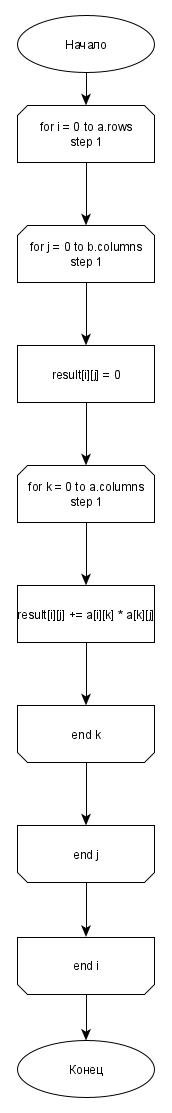
\includegraphics[width=0.7\linewidth]{C:/Users/User/Desktop/Studing/Analysis_Algorithm/lab_02/Отчет/Схемы/simple}
		\caption{}
		\label{fig:simple}
	\end{figure}
	
	
	\subsubsection{Алгоритм Винограда}
	
	\begin{figure}[]
		\centering
		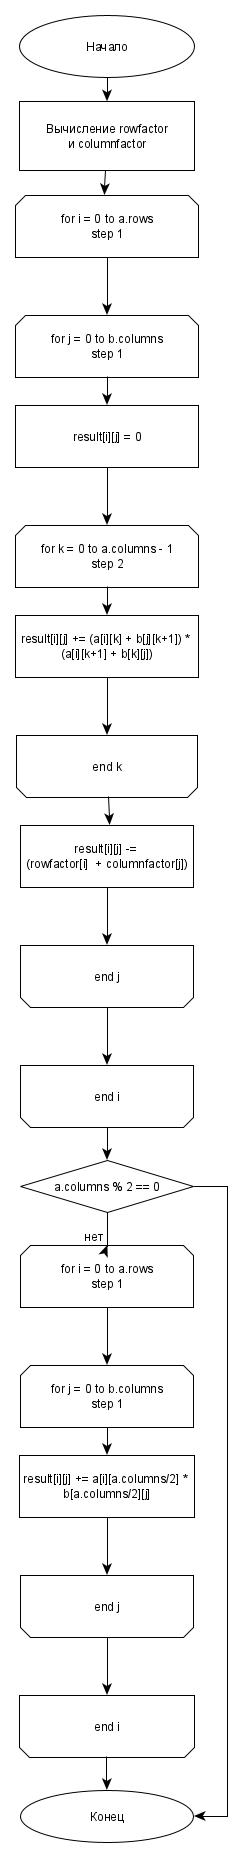
\includegraphics[width=0.7\linewidth]{C:/Users/User/Desktop/Studing/Analysis_Algorithm/lab_02/Отчет/Схемы/vinograd}
		\caption{}
		\label{fig:vinograd}
	\end{figure}
	
	
	\subsubsection{Rowfactor}
	
	\begin{figure}[]
		\centering
		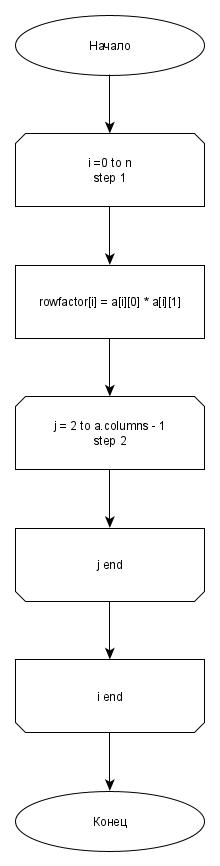
\includegraphics[width=0.7\linewidth]{C:/Users/User/Desktop/Studing/Analysis_Algorithm/lab_02/Отчет/Схемы/rowfactor}
		\caption{}
		\label{fig:rowfactor}
	\end{figure}
	
	
	\newpage
	\section{Технологический раздел}
	
	\newpage
	\section{Исследовательский раздел}
	
	\newpage
	\section{Вывод}
	
	\newpage
	\section{Заключение}